\documentclass[10pt,paper=letter]{scrartcl}
\usepackage[alttitle]{cjquines}

\begin{document}

\title{VCSMS PRIME}
\subtitle{Program for Inducing Mathematical Excellence}
\author{Session 3: Combinatorial Principles}
\date{September 21, 2017}

\maketitle
\setlength{\unitlength}{1in}
\begin{picture}(0,0)
  \put(5.5,0.5){\hbox{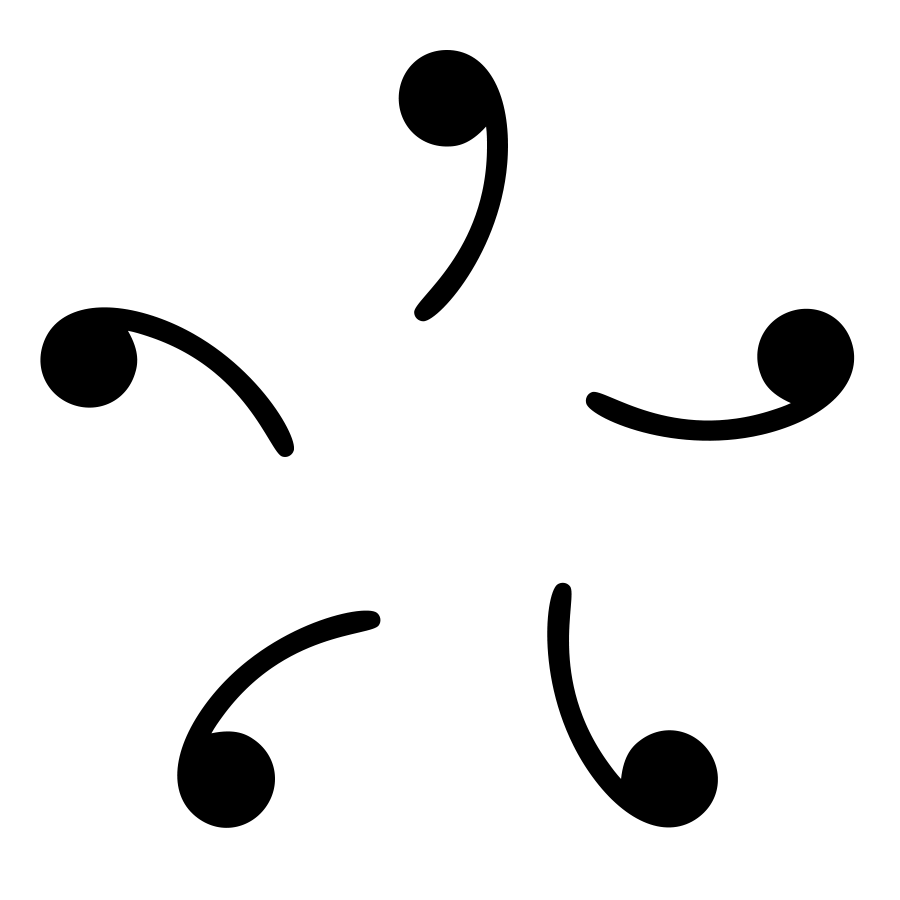
\includegraphics[width=0.9in]{logo.png}}}
\end{picture}
\vspace{-3.5em}

\subsubsection*{Lecture problems}

\begin{enumerate}
  \item (QII1) I have $2016$ identical marbles. I plan to distribute them equally into one or more identical containers. How many ways can this be done if I have an unlimited number of containers?
  \item (QI13) How many three-digit numbers have distinct digits that add up to $21$?
  \item (QIII2) Using the numbers $1, 2, 3, 4, 5, 6$ and $7,$ we can form $7! = 5040$ 7-digit numbers in which the 7 digits are all distinct. If these numbers are listed in increasing order, find the $2016$th number in the list.
  \item A set of points is chosen on the circumference of a circle so that the number of different triangles with all three vertices among the points is equal to the number of pentagons with all five vertices in the set. How many points are there?
  \item Compute $\binom{1000}{0} + \binom{1000}{2} + \binom{1000}{4} + \cdots + \binom{1000}{1000}$.
  \item (AI15) How many numbers between $1$ and $2016$ are divisible by exactly one of $4, 6,$ or $10$?
  \item (QII9) How many ordered triples of positive integers $(x, y, z)$ are there such that $x+y+z = 20$ and two of $x, y, z$ are odd?
\end{enumerate}

\subsubsection*{Counting is multiplication}

\begin{itemize}
  \item The number of ways to choose in a series of independent choices is the product of the number of choices. When it's in a row (or a circle, or whatever) it's called a \emph{permutation}.
  \item Problem 1: The formula for the number of divisors is $\prod (e_i + 1)$ because for each prime $p_i$, a divisor can have either $p_i^0, p_i^1, p_i^2, \ldots, p_i^{e_i}$ as a factor.
  \item Problem 2: Sometimes you just have to count brute force. Then multiply by $3!$ to account for the number of arrangements, but be careful with zero. General rule: $n!$ ways to arrange $n$ items in a row.
  \item Problem 3: This is like ``the permutations of VALMASCI are sorted alphabetically, what is the $n$th word in the list?'' This is called \emph{lexicographical order}, and you count by going left-to-right, slot-by-slot. How many with first digit $1$? First digit $2$? Then if you go over $2016$ you move to the next digit.
\end{itemize}

\subsubsection*{Counting is division}

\begin{itemize}
  \item When order matters, it's a permutation, but when it doesn't it's a combination. Sometimes we \emph{overcount}, and we want to count things as the same. How many ways to arrange letters in PHILIPPINES? 
  \item Permutations on a circle: divide by $n$. With reflections: divide by $2$.
  \item When order doesn't matter, it's called \emph{combination}: divide by $k!$. This gives binomial coefficients $\binom{n}{k}$.
  \item Problem 4: A triangle is defined by its three vertices, same for a pentagon, so $\binom{n}{3} = \binom{n}{5}$. Cancel.
  \item Why ``binomial coefficient''? Because it's the coefficients in $(x + y)^n$. 
  \item Problem 5: What happens when we expand $(1 + 1)^{1000}$ and $(1 - 1)^{1000}$ using the binomial theorem?
\end{itemize}

\subsubsection*{Counting is addition (and subtraction)}

\begin{itemize}
  \item Draw Venn diagrams and add and subtract. For PIE, the pattern is add, subtract, add, subtract, add, subtract. 
  \item Problem 6: Add divisble by $4, 6, 10$, subtract twice divisible by $\text{lcm}(4, 6) = 12, \text{lcm}(4, 10) = 20, \text{lcm}(6, 10) = 30$, add thrice divisible by $\text{lcm}(4, 6, 10) = 60$.
\end{itemize}

\subsubsection*{Counting is bijection}

\begin{center}
\def\arraystretch{2}
  \begin{tabular}{l|l|l|l|l}
    $b$ balls & $u$ urns & no restriction & at most 1 & at least 1 \\ \hline
    D & D & & & (hard) \\ \hline
    I & D & & & \\ \hline
    D & I & (hard) & & (hard) \\ \hline
    I & I & (hard) & & (hard)
  \end{tabular}
\end{center}

\begin{itemize}
  \item Twelvefold way: distinguishable vs indistinguishable balls (2), distinguishable vs indistinguishable urns (2), no restriction vs at most one ball in each urn vs at least one ball in each urn (3).
  \item We know how to do five out of twelve:
  \begin{itemize}
    \item How many ways to give three different candies to five children? ($5^3$)
    \item How many ways to give three different candies to five children, so that each child gets at most one candy? ($5\times 4 \times 3$)
    \item How many ways to give three identical candies to five children, so that each child gets at most one candy? ($\binom{5}{3}$)
    \item How many ways to place three different candies in five identical pouches, so that each pouch has at most one candy? ($1$)
    \item How many ways to place three identical candies, in five identical pouches, so that each pouch has at most one candy? ($1$)
  \end{itemize}
  \item Another five out of twelve have no simple formula, and should be done manually.
  \item The remaining two can be done with balls and urns arguments:
  \begin{itemize}
    \item How many ways to give three identical candies to five children? ($\binom{3+5}{3}$)
    \item How many ways to give three identical candies to two children, so each child gets at least one candy? ($\binom{3-1}{2-1}$)
  \end{itemize}
  \item Appears in lots of ways:
  \begin{itemize}
    \item $w+x+y+z = c$ for nonnegative or positive integers.
    \item How many ways to roll $5$ dice so the sum is $16$?
    \item Problem 7: There are $\binom{3}{2}$ ways to pick the two odd numbers. Rewrite as $2a+1, 2b+1, 2c$, and then do balls and urns, then remember to multiply by $\binom{3}{2}$.
    \item Selecting $6$ cookies out of $3$ different kinds, when you have unlimited supplies of each kind.
    \item Number of $7$-digit numbers with digits in increasing order.
    \item How many ways to arrange $3$ maple trees, $4$ oak trees and $5$ birch trees in a row so no two birch trees are adjacent?
  \end{itemize}
\end{itemize}

\end{document}
